% ------------------------------------------------------------------------------
% TYPO3 CMS 8.3 - What's New - Chapter "Changements en profondeur" (French Version)
%
% @author	Patrick Lobacher <patrick@lobacher.de> and Michael Schams <schams.net>
% @license	Creative Commons BY-NC-SA 3.0
% @link		http://typo3.org/download/release-notes/whats-new/
% @language	French
% ------------------------------------------------------------------------------
% LTXE-CHAPTER-UID:		5ebcecbe-66abfa57-cf38bc00-aa637965
% LTXE-CHAPTER-NAME:	Changements en profondeur
% ------------------------------------------------------------------------------

\section{Changements en profondeur}
\begin{frame}[fragile]
	\frametitle{Changements en profondeur}

	\begin{center}\huge{Chapitre 3~:}\end{center}
	\begin{center}\huge{\color{typo3darkgrey}\textbf{Changements en profondeur}}\end{center}

\end{frame}

% ------------------------------------------------------------------------------
% LTXE-SLIDE-START
% LTXE-SLIDE-UID:		a815951f-9b306772-bd0339e1-5d4308d6
% LTXE-SLIDE-ORIGIN:	bd33b29d-c20d1765-f923f78e-43bfb0bf English
% LTXE-SLIDE-TITLE:		Feature #74365: Add Linkservice for Unified Referencing Syntax (1)
% LTXE-SLIDE-REFERENCE:	Feature-74365-LinkServiceForUnifiedReferencingSyntax.rst
% ------------------------------------------------------------------------------
\begin{frame}[fragile]
	\frametitle{Changements en profondeur}
	\framesubtitle{Ajout de Linkservice pour une syntaxe de référence unifiée (1)}

	\begin{itemize}

		\item Les ressources dans TYPO3 étaient référencées en utilisant des formes multiples et différentes dans le passé.

		\item TYPO3 supporte maintenant une manière moderne et à l'épreuve du temps de référencer les ressources utilisant
			une syntaxe extensible et expressive facile à comprendre.

		\item Les prochaines diapositives expliquent la syntaxe en utilisant le lien de page simple~:

			\begin{lstlisting}
				t3://page?uid=13&campaignCode=ABC123
			\end{lstlisting}

	\end{itemize}

\end{frame}

% ------------------------------------------------------------------------------
% LTXE-SLIDE-START
% LTXE-SLIDE-UID:		7ea1bc9f-42ee436a-03391d87-f4e879f3
% LTXE-SLIDE-ORIGIN:	95f9a663-ea2155a1-5635728b-77a8995c English
% LTXE-SLIDE-TITLE:		Feature #74365: Add Linkservice for Unified Referencing Syntax (2)
% LTXE-SLIDE-REFERENCE:	Feature-74365-LinkServiceForUnifiedReferencingSyntax.rst
% ------------------------------------------------------------------------------
\begin{frame}[fragile]
	\frametitle{Changements en profondeur}
	\framesubtitle{Ajout de Linkservice pour une syntaxe de référence unifiée (2)}

	\begin{itemize}

		\item La syntaxe consiste en trois parties~:

			\begin{itemize}

				\item L'espace de nom (\texttt{t3://})\newline
		   			L'espace de nom est fixé à \texttt{t3://} pour assurer l'exécution du «~LinkService~» pour analyser l'URN.
					\newline
				\item La clé de gestionnaire de ressources (\texttt{page})\newline
   					La clé de gestionnaire de ressources l'identifie dans la liste de ceux disponibles dans TYPO3.
					Lors de la rédaction, les gestionnaires suivants existent~: \texttt{page}, \texttt{file} et \texttt{folder}.\newline
					Des clés supplémentaires sont à ajouter au tableau associatif, avec comme clé, la clé du gestionnaire, et
					comme valeur, une classe implémentant LinkHandlerInterface~:\newline
					\texttt{\$TYPO3\_CONF\_VARS['SYS']['linkHandler']}

			\end{itemize}

	\end{itemize}

\end{frame}

% ------------------------------------------------------------------------------
% LTXE-SLIDE-START
% LTXE-SLIDE-UID:		f5694ef5-be60529e-e2166e1c-b9133993
% LTXE-SLIDE-ORIGIN:	77a8995c-ea2155a1-95f9a663-5635728b English
% LTXE-SLIDE-TITLE:		Feature #74365: Add Linkservice for Unified Referencing Syntax (3)
% LTXE-SLIDE-REFERENCE:	Feature-74365-LinkServiceForUnifiedReferencingSyntax.rst
% ------------------------------------------------------------------------------
\begin{frame}[fragile]
	\frametitle{Changements en profondeur}
	\framesubtitle{Ajout de Linkservice pour une syntaxe de référence unifiée (3)}

	\begin{itemize}

		\item …et la 3ième partie~:

			\begin{itemize}

				\item Paramètres de la ressource (\texttt{?uid=13\&campaignCode=ABC123})\newline
					Ce sont les paramètres d'identification spécifiques de la ressource pour les gestionnaires.
					Notez qu'ils peuvent contenir des paramètres additionnels pour configurer le comportement des
					gestionnaires.

			\end{itemize}

	\end{itemize}

\end{frame}

% ------------------------------------------------------------------------------
% LTXE-SLIDE-START
% LTXE-SLIDE-UID:		80d26608-b6c71a5b-2e4dd287-e773e3c4
% LTXE-SLIDE-ORIGIN:	af8e73a4-2b315873-bb6e55e4-c0cd82b5 English
% LTXE-SLIDE-TITLE:		#76008 and #76458: DebuggerUtility::var_dump (1)
% LTXE-SLIDE-REFERENCE:	Feature-76008-PropertyVisibilityToDebuggerUtilityvar_dump.rst
% LTXE-SLIDE-REFERENCE:	Feature-76458-LetDebuggerUtilityRenderClosures.rst
% ------------------------------------------------------------------------------
\begin{frame}[fragile]
	\frametitle{Changements en profondeur}
	\framesubtitle{\texttt{DebuggerUtility::var\_dump} (1)}

	\begin{itemize}

		\item L'information de visibilité des propriétés est ajoutée à \texttt{DebuggerUtility::var\_dump()}
			\newline
			pour chaque propriété d'objet dans le déchargement

		\item Si une fermeture fait partie de l'objet déchargé, le code source de la fermeture est aussi affiché

	\end{itemize}

	\tabto{0.75cm}\textit{Voir l'exemple dans la diapositive suivante}

\end{frame}

% ------------------------------------------------------------------------------
% LTXE-SLIDE-START
% LTXE-SLIDE-UID:		bbdf22f8-e6ef2c26-0e85b521-e87173a0
% LTXE-SLIDE-ORIGIN:	bb6e55e4-2b315873-c0cd82b5-af8e73a4 English
% LTXE-SLIDE-TITLE:		#76008 and #76458: DebuggerUtility::var_dump (2)
% LTXE-SLIDE-REFERENCE:	Feature-76008-PropertyVisibilityToDebuggerUtilityvar_dump.rst
% LTXE-SLIDE-REFERENCE:	Feature-76458-LetDebuggerUtilityRenderClosures.rst
% ------------------------------------------------------------------------------
\begin{frame}[fragile]
	\frametitle{Changements en profondeur}
	\framesubtitle{\texttt{DebuggerUtility::var\_dump} (2)}

	\begin{figure}
		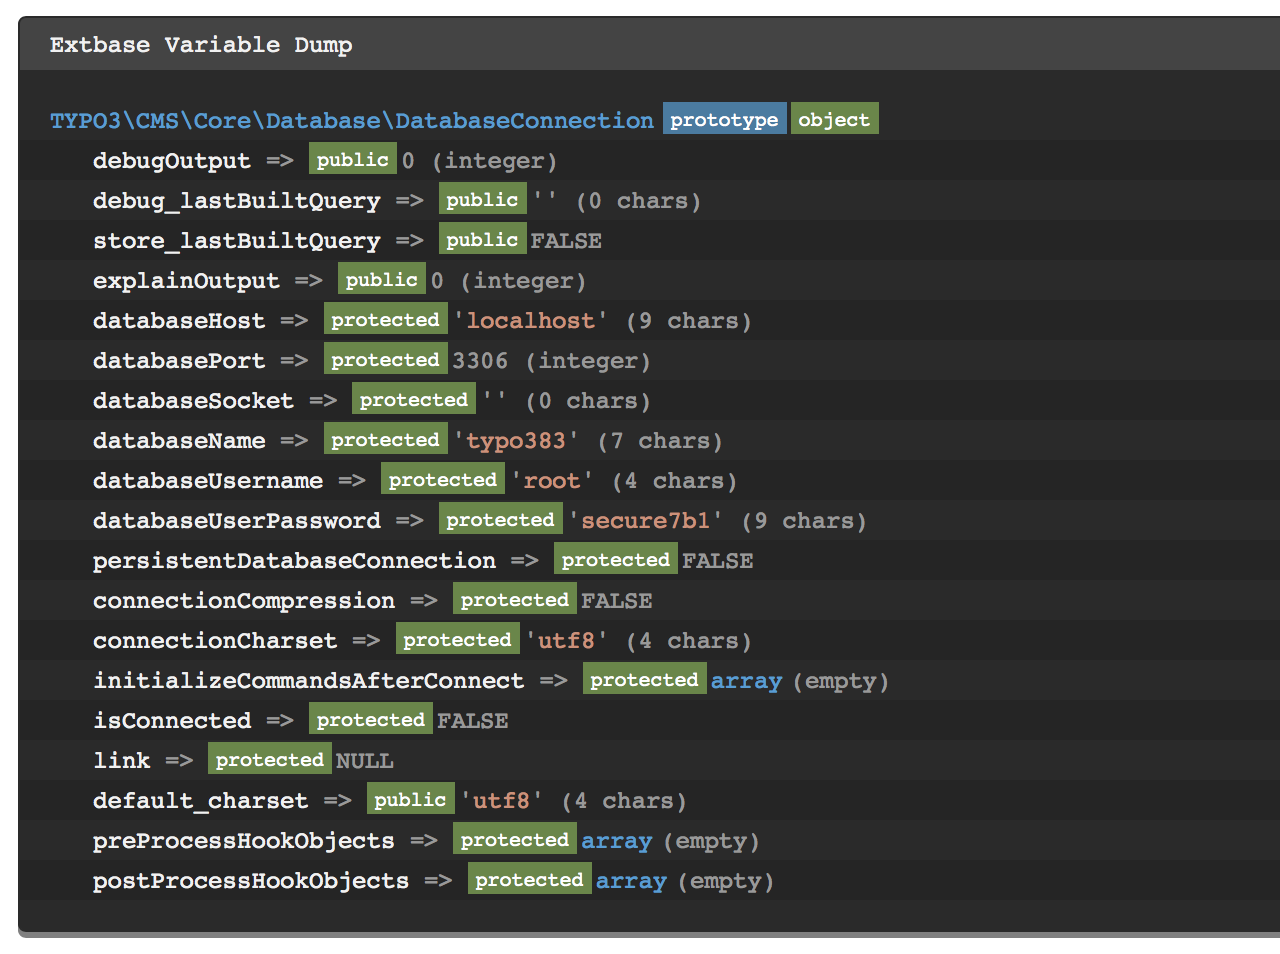
\includegraphics[width=0.65\linewidth]{InDepthChanges/76008.png}
	\end{figure}

\end{frame}

% ------------------------------------------------------------------------------
% LTXE-SLIDE-START
% LTXE-SLIDE-UID:		7f3f31fe-51405ea8-df8e0cca-b6a760de
% LTXE-SLIDE-ORIGIN:	2b74180d-e68ba0c2-8826a2cf-8498f977 English
% LTXE-SLIDE-TITLE:		!Breaking: #73461 - Import module disabled for non admin users
% LTXE-SLIDE-REFERENCE:	!Breaking-73461-ImportModuleDisabledForNonAdminUsers.rst
% ------------------------------------------------------------------------------
\begin{frame}[fragile]
	\frametitle{Changements en profondeur}
	\framesubtitle{Module d'importation désactivé pour les non-administrateurs}

	\begin{itemize}

		\item Le module d'importation de \texttt{EXT:impexp} est désactivé pour les utilisateurs non-administrateurs par défaut

		\item Pour ceux qui en ont le besoin, l'option de configuration TSconfig utilisateur suivante
			est à définir~:\newline
			\texttt{options.impexp.enableImportForNonAdminUser = 1}

			\vspace{0.5cm}

			\begingroup
				\color{typo3red}
				Attention~: ceci peut devenir un problème sérieux de sécurité pour les versions 6.2 et 7.6 de TYPO3
				et ne devrait être activé que pour les utilisateurs Backend \textit{de confiance}.
			\endgroup

	\end{itemize}

\end{frame}

% ------------------------------------------------------------------------------
% LTXE-SLIDE-START
% LTXE-SLIDE-UID:		ded0335f-5d276334-eff6d2eb-d1eb0016
% LTXE-SLIDE-ORIGIN:	bac423cc-ba00db30-e1538b7f-25749380 English
% LTXE-SLIDE-TITLE:		Hooks and Signals (1)
% LTXE-SLIDE-REFERENCE:	!Feature-76209-HookToRegisterCustomResultBrowsersInAbstractPlugin.rst
% ------------------------------------------------------------------------------
\begin{frame}[fragile]
	\frametitle{Changements en profondeur}
	\framesubtitle{Hooks et Signals (1)}

	% decrease font size for code listing
	\lstset{basicstyle=\tiny\ttfamily}

	\begin{itemize}

		\item Un nouveau hook permet d'inscrire une implémentation personnalisée du navigateur de résultats

		\item Cette approche permet de surcharger l'implémentation par défaut de
			\texttt{AbstractPlugin::pi\_list\_browseresults()}
			pour toutes les extensions ou quelques-unes.

		\item Le hook s'inscrit dans \texttt{ext\_localconf.php}~:

			\begin{lstlisting}
				$GLOBALS['TYPO3_CONF_VARS']['SC_OPTIONS']
				  [\TYPO3\CMS\Frontend\Plugin\AbstractPlugin::class]['pi_list_browseresults'][1463475262] =
				  \Vendor\ExtensionKey\Hook\ResultBrowserHook::class
			\end{lstlisting}

	\end{itemize}

\end{frame}


% ------------------------------------------------------------------------------
% LTXE-SLIDE-START
% LTXE-SLIDE-UID:		3d3e9d3a-15ef5d05-ab1f039b-6b4c796c
% LTXE-SLIDE-ORIGIN:	82c70aee-3b375252-6cac0ad6-b385b95f English
% LTXE-SLIDE-TITLE:		Hooks and Signals (2)
% LTXE-SLIDE-REFERENCE:	!Feature-76259-IntroduceBuildQueryParametersPostProcessHook.rst
% ------------------------------------------------------------------------------
\begin{frame}[fragile]
	\frametitle{Changements en profondeur}
	\framesubtitle{Hooks et Signals (2)}

	% decrease font size for code listing
	\lstset{basicstyle=\tiny\ttfamily}

	\begin{itemize}

		\item Avec la migration à Doctrine, le hook \texttt{buildQueryParameters} est introduit dans la classe
			\texttt{DatabaseRecordList}.

		\item Ce hook remplace le hook \texttt{makeQueryArray} de la méthode dépréciée
			\texttt{AbstractDatabaseRecordList::makeQueryArray}.

		\item L'usage de ce nouveau hook permet de modifier les paramètres de la requête à la base de données
		 	pour les enregistrements à afficher dans la vue liste d'enregistrements

		\item Le hook s'inscrit dans \texttt{ext\_localconf.php}:

			\begin{lstlisting}
				$GLOBALS['TYPO3_CONF_VARS']['SC_OPTIONS']
				  [\TYPO3\CMS\Recordlist\RecordList\DatabaseRecordList::class]['buildQueryParameters'][]
			\end{lstlisting}

		\item …et implémente la méthode publique \texttt{buildQueryParametersPostProcess}

	\end{itemize}

\end{frame}

% ------------------------------------------------------------------------------
% LTXE-SLIDE-START
% LTXE-SLIDE-UID:		a503e0e0-1789f18e-3ed4d386-5f8246eb
% LTXE-SLIDE-ORIGIN:	73d888ce-a14c0f6a-d4dec5fb-f7368bb6 English
% LTXE-SLIDE-TITLE:		!Breaking: #76108 - Replace ExtJS category tree with D3 and SVG
% LTXE-SLIDE-TITLE:		!Feature: #77349 - Additional locations for extension icons
% LTXE-SLIDE-TITLE:		!Feature: #77481 - Add possibility to define a favicon for the backend
% LTXE-SLIDE-REFERENCE:	!Breaking-76108-ReplaceExtJSCategoryTreeWithD3AndSVG.rst
% LTXE-SLIDE-REFERENCE:	!Feature-77349-AdditionalLocationsForExtensionIcons.rst
% LTXE-SLIDE-REFERENCE:	!Feature-77481-AddPossibilityToDefineAFaviconForTheBackend.rst
% ------------------------------------------------------------------------------
\begin{frame}[fragile]
	\frametitle{Changements en profondeur}
	\framesubtitle{Divers}

	\begin{itemize}

		\item Rendus SVGs et D3

			\begin{itemize}
				\item Avec le retrait de ExtJS du noyau de TYPO3, l'arborescence dans les formulaires d'édition est retravaillée
				\item Le rendu est basé sur SVGs et D3, fournissant un gain de performances
				\item Le retravaille de l'arborescence des pages de la même manière est prévu rapidement
			\end{itemize}

		\item Les icônes d'extension s'enregistrent dans le dossier suivant~:\newline
			\small
				\texttt{Resources/Public/Icons/<filename>}
				(où <filename> est l'un de~: \texttt{Extension.png}, \texttt{Extension.svg} ou \texttt{Extension.gif})
			\normalsize

		\item La nouvelle option \texttt{backendFavicon} dans la configuration du Gestionnaire d'Extensions permet
			de changer l'icône de favoris du backend.

	\end{itemize}

\end{frame}

% ------------------------------------------------------------------------------
